\section{Fourierreihe}
  	$$\boxed{f(t) = \sum\limits_{k = -\infty}^{\infty} c_k \cdot e^{j k \omega_1
  	t}}= \boxed{\sum\limits_{k = 0}^{\infty} \left(c_k \cdot e^{j k \omega_1
  	t} + \overline{c_k} \cdot e^{-j k \omega_1t}\right)}$$
  	$$\boxed{f(t) = \frac{a_0}{2} + \sum\limits_{k=1}^{\infty} \left[a_k \cos(k
  	\omega_1 t) + b_k \sin(k \omega_1 t)\right]}=\boxed{\frac{A_0}{2} +
  	\sum\limits_{k=1}^{\infty} A_k \cos(k \omega_1 t + \varphi_k)} \quad k\in
  	\mathbb{Z}, \quad \omega_1=\frac{2 \pi}{T}=2 \pi f$$	
	
	$$\boxed{c_k=\overline{c_{-k}}=\frac{1}{T}\int_0^T{f(t)\cdot
	e^{-jk\omega_1
	t}dt} \; ; \; c_0 \neq a_0} \qquad \boxed{a_0 = \frac{2}{T}\int\limits_0^{T}
	f(t)dt, \quad a_k = \frac{2}{T}\int\limits_0^{T} f(t)\cos(k \omega_1 t) dt, \quad b_k =
	\frac{2}{T}\int\limits_0^{T} f(t)\sin(k \omega_1 t) dt}$$

	$a_0$, $c_0$, $A_0$ sind \textit{Konstanten}, $\omega_1$ ist die
	\textit{Grundkreisfrequenz}, $a_k$ und $b_k$ sind die \textit{reellen
	Koeffizienten}, $c_k$ ist der \textit{komplexe Koeffizient}, $A_k$ ist die
	\textit{Amplitude} und $\varphi_k$ ist die \textit{Phase}.\\
	\fbox{
	\begin{tabular}{p{9cm}p{9cm}}
		$a_k = c_k + \bar{c_k} = 2\Real(c_k) = A_k \cos(\varphi_k)$ &
		$b_k = j(c_k + \bar{c_k}) = -2\Imag(c_k) = -A_k \sin(\varphi_k)$ \\ \\
		$c_k = \frac{a_k-jb_k}{2} = \frac{A_k}{2} e^{j\varphi_k} = \frac1T
		F(j k \omega)$ &
		$c_{-k} = \overline{c_k} = \frac{a_k+jb_k}{2} = \frac{A_k}{2} e^{-j\varphi_k}$ \\ \\
		$A_k = 2|c_k| = \sqrt{a_k^2+b_k^2}$ & $\varphi_k =  \arg(c_k)$\\
	\end{tabular}}\\

	\textbf{Berechnung von $\varphi_k$ aus $a_k$ und $b_k$}\\
	\begin{tabular}{p{4cm}p{4cm}p{3cm}p{3.5cm}}
		$a_k> 0:$ & $\varphi_k = -\arctan(\frac{b_k}{a_k})$ &
		$a_k<0:$ &	$\varphi_k = -\arctan(\frac{b_k}{a_k}) + \pi$\\
		$a_k = 0 \wedge b_k > 0:$ &	$\varphi_k = -\frac{\pi}{2}$ &
		$a_k = 0 \wedge b_k < 0:$ &	$\varphi_k = \frac{\pi}{2}$\\
		$a_k = 0 \wedge b_k = 0:$ &	$\varphi_k = \text{nicht definiert}$
	\end{tabular}

	\subsection{Symmetrie}
		\begin{tabular}{|p{4.3cm}|p{4.3cm}|p{4.4cm}|p{4.4cm}|}
         	\hline
        	\textbf{gerade Funktion} & \textbf{ungerade Funktion} &
        	\textbf{Halbperiode 1} & \textbf{Halbperiode 2}\\
        	\hline
        	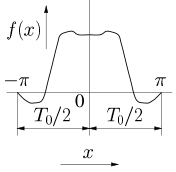
\includegraphics[width=3cm]{./bilder/gerade_funktion.png}&
        	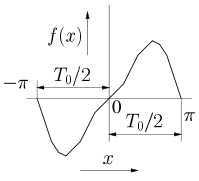
\includegraphics[width=3cm]{./bilder/ungerade_funktion.png}&   
 			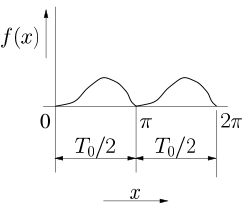
\includegraphics[width=3cm]{./bilder/halbperiode_1.png}&   
			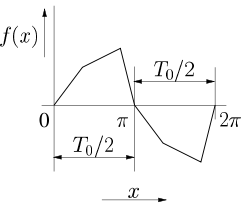
\includegraphics[width=3cm]{./bilder/halbperiode_2.png}\\
			\hline & & & \\			
   			$f(-t)=f(t)$ & $f(-t)=-f(t)$ & $f(t)=f(t+\pi)$ & $f(t)=-f(t+\pi)$\\
   			$b_k=0$ & $a_k=0$ & $a_{2k+1}=0$ & $a_{2k}=0$\\
   			$a_k = \frac{4}{T} \int\limits_0^{\frac{T}{2}} f(t) \cdot \cos(k \omega_1
   			t) dt$ &
   			$b_k =  \frac{4}{T} \int\limits_0^{\frac{T}{2}} f(t) \cdot
			\sin(k \omega_1 t) dt$ &
			$b_{2k+1}=0$ & $b_{2k}=0$\\
			\hline
      	\end{tabular}

	\subsection{Rechtecksignale}
	$$a_k=\frac{2}{T}\int\limits_{-t_1/2}^{t_1/2}A\cos\left(\frac{2\pi k}{T}t\right)dt=
	\left .\frac{2AT}{2\pi T k}\sin \left(\frac{2\pi k}{T}t\right)\right |_{-t_1/2}^{t_1/2}=
	\frac{2A}{\pi k}\sin\left(\frac{\pi t_1}{T}k\right)$$
	F"ur Verh"altnisse $\frac{T}{ggT(t_1,T)}=n\in\mathbb{N}$ verschwinden die
	$n.$ Harmonische und deren Vielfache.\\
	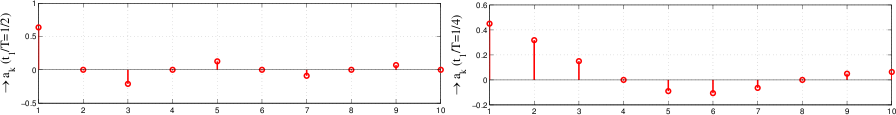
\includegraphics[width=19cm]{./bilder/fourierreihe-rechteck.png}